%% paper/sections/results.tex
%% Draft only. All three pre-registered structural hypotheses are null; no
%% hedging toward a positive reading anywhere below. Every number traced via
%% inline LaTeX comment.
\label{sec:results}

\subsection{Structural Hypotheses: All Three Null}
Three pre-registered hypotheses were evaluated against locked recipes, test
touched exactly once per condition/seed
(\S\ref{sec:pre-registration}). All three are null.

\textbf{H1, MELD (persistence).}
%% outputs/meld_phase4_statistics.json: h1_persistence.mean_margin, ci_low, ci_high
$A1 - A2 = 0.0340$, 95\% CI $[0.0203, 0.0480]$. The CI excludes zero, but the
point estimate is below $\text{EFFECT\_FLOOR}{=}0.04$. \textbf{Not
supported.} Per the frozen decision rule, this is reported as underpowered,
not as evidence that persistence has no effect.

\textbf{H2, MELD (entity structure).}
%% outputs/meld_phase4_statistics.json: h2_entity_structure.mean_margin, ci_low, ci_high
$A1 - A0 = 0.0315$, 95\% CI $[0.0159, 0.0470]$. Same pattern: CI excludes
zero, point estimate below the floor. \textbf{Not supported.} With neither H1
nor H2 clearing $\text{EFFECT\_FLOOR}$, none of the three branches in the
MELD decision rule fire
%% outputs/meld_phase4_statistics.json: decision.branch == null
--- reported as such, not forced into the nearest branch.

\textbf{H2, DAiSEE (replication).}
%% outputs/daisee_phase4_statistics.json: h2_item_paired_bootstrap.mean_margin, ci_low, ci_high
$A1 - A0 = 0.0037$, 95\% CI $[-0.0199, 0.0264]$, primary metric (macro-F1,
classes 1--3, \S\ref{sec:pre-registration}). The CI includes zero.
\textbf{Not supported} --- branch (b), null/underpowered, per the frozen
rule
%% outputs/daisee_phase4_statistics.json: decision.branch == "b"
.

\textbf{These are two different flavors of null, and the difference matters
for how they're read.} MELD's H1 and H2 margins are positive with CIs that
exclude zero --- a real, non-noise signal that simply does not clear the
pre-registered bar. DAiSEE's H2 margin is indistinguishable from zero by
every measure computed (\S\ref{sec:sensitivity}). MELD's H2 (0.0315) does
not replicate as DAiSEE's H2 (0.0037): the same structural comparison,
entity-localized tokens against a matched-budget spatial grid, produces a
detectable-but-underpowered gap on multi-party television video and no
detectable gap at all on single-subject webcam video. We report this as a
\textbf{failure to replicate}, not as a stronger MELD finding standing
uncontested.

One \emph{post hoc, untested} hypothesis for the divergence, offered here
explicitly as such and not fit to any data beyond what is already reported:
DAiSEE's $E{=}1$ crop is a single dominant-subject region that likely already
covers most of the frame's informative content, since webcam framing
centers the subject by construction; MELD's multi-party wide shots contain
substantially more frame area outside any one speaker, so entity-localized
cropping there discards more distractor content than it does on DAiSEE. If
this is right, the entity-vs-grid gap should scale with how much of the
frame a matched-budget grid wastes on non-entity content --- a claim this
paper does not test.

\subsection{Purity-Stratified Secondary Analysis (MELD)}
Pre-registered before computation, secondary to the branch decision above:
%% outputs/meld_phase4_purity_stratified.json: tercile_p33, tercile_p67, tercile_counts
MELD test clips were split into purity terciles (silhouette-score-based
identity-clustering quality, cutpoints $0.8008$/$0.9067$, 870 clips each) and
H1's margin recomputed within each. If persistence's pooled null reflected
imperfect identity recovery (\S\ref{sec:pre-registration}'s 62.2\% clustering
purity) rather than a true absence of effect, the margin should grow
monotonically with purity. It does not:
%% outputs/meld_phase4_purity_stratified.json: margins_low_mid_high, monotone
margins are $0.0377$ (low purity), $0.0264$ (mid), $0.0389$ (high) --- not
monotone. This argues against ``identity wasn't recovered well enough to
tell'' as the explanation for the pooled null, without resolving it into a
positive finding either.

\subsection{Sensitivity and Robustness}
\label{sec:sensitivity}
\begin{figure}[t]
  \centering
  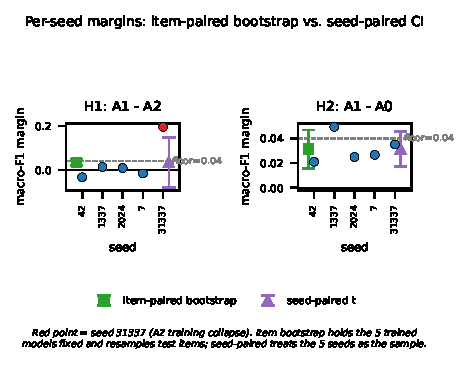
\includegraphics[width=\linewidth]{figures/fig4_seed_margin_divergence.pdf}
  \caption{Per-seed H1/H2 margins (MELD), item-paired bootstrap vs.\
    seed-paired $t$ interval. Seed 31337 (red, H1 panel) is A2's training
    collapse; the two interval estimates diverge for H1 and agree for H2.}
  \label{fig:seed-margin}
\end{figure}
\textbf{Leave-one-seed-out (MELD).} Dropping seed 31337 --- which collapsed
during A2 training (dev macro-F1 falling to majority-class level in the
final two epochs, visible in both train and dev curves at that seed) ---
flips H1's margin sign
%% outputs/meld_phase4_posthoc_analysis.json: leave_one_out_h1, seed 31337 entry
(from $+0.034$ pooled to $-0.006$ with that seed excluded); dropping any of
the other four seeds individually keeps H1 close to or above $0.04$
%% outputs/meld_phase4_posthoc_analysis.json: leave_one_out_h1, all five drop-one entries (0.0390-0.0508 excluding the 31337 drop)
(0.0390--0.0508; three of the four stay above the floor, dropping seed 1337
alone brings it to 0.0390, just under). H2 is stable under every
leave-one-out fold. This is diagnostic, not a revision: the pre-registered
5-seed result stands.

\textbf{Item-paired vs.\ seed-paired tests diverge for H1, agree for H2
(MELD).} A seed-paired $t$-test on H1's five per-seed margins gives
%% outputs/meld_phase4_posthoc_analysis.json: seed_paired_h1.paired_t_p, wilcoxon_p
$p{=}0.457$ (Wilcoxon $p{=}1.0$) --- no significant effect --- against the
item-paired bootstrap's zero-excluding CI above. For H2, the seed-paired test
gives
%% outputs/meld_phase4_posthoc_analysis.json: seed_paired_h2.paired_t_p, wilcoxon_p
$p{=}0.0034$ (Wilcoxon $p{=}0.0625$, the smallest attainable at $n{=}5$),
agreeing with the item-paired result. The divergence for H1 is explained by
what each test conditions on: the item-paired bootstrap holds the five
already-trained models fixed and asks only whether the margin survives
resampling test items, so a single collapsed seed's degenerate predictions
stay degenerate in every resample; the seed-paired test treats the five
per-seed margins as the sample, so that same collapse dominates the
between-seed variance directly. H2 has no comparable outlier seed, and the
two tests agree.

\textbf{Item-paired and seed-paired agree for DAiSEE's H2.} Paired $t$
%% outputs/daisee_phase4_statistics.json: h2_seed_paired.paired_t_p, wilcoxon_p
$p{=}0.793$, Wilcoxon $p{=}0.8125$ --- both consistent with the item-paired
CI including zero. No seed behaved like MELD's 31337; this null is not an
artifact of one bad run.

\subsection{Ablations}
%% results/summary.csv: A3, A4, A5, mask_only rows (macro_f1_mean +/- macro_f1_std)
A3 (temporal-only) reaches $0.4032{\pm}0.0431$ and A4 (social-only) reaches
$0.4111{\pm}0.0311$, both close to A1's $0.4040{\pm}0.0077$
(\S\ref{sec:pre-registration}'s primary condition) --- neither attention axis
alone is doing dramatically more or less than the combination. A5
(mean-pooled entities, no attention at all,
%% results/summary.csv: A5 row
$0.3901{\pm}0.0081$) is within noise of A0
%% results/summary.csv: A0 row
($0.3725{\pm}0.0092$) and not far below A1, consistent with
\S\ref{sec:efficiency}'s finding that attention structure contributes little
compute and, on this evidence, not dramatically more accuracy either.
Mask-only
%% results/summary.csv: mask_only row
($0.2459{\pm}0.0021$) fails to clear the trivial-feature-probe floor
($0.3648$, \S\ref{sec:pre-registration}) at every seed --- who is on screen,
alone, does not predict sentiment on MELD.

\subsection{Efficiency}
\label{sec:efficiency}
\begin{figure}[t]
  \centering
  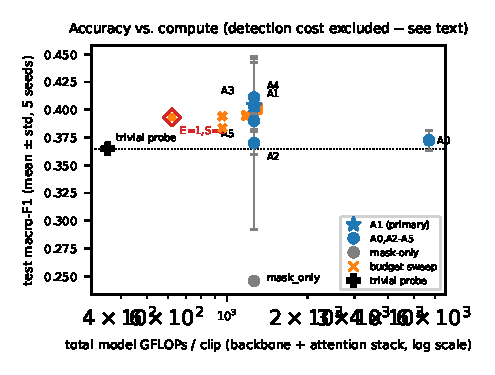
\includegraphics[width=\linewidth]{figures/fig3_pareto_gflops.pdf}
  \caption{Accuracy vs.\ latency by hardware regime (MELD). No panel mixes
    GPU- and CPU-measured numbers. Regime A (GPU-only) is not measured:
%% outputs/meld_phase6_gpu_detection_attempt.json: root_cause
    \texttt{onnxruntime-gpu} 1.28.0's prebuilt wheel requires CUDA 13's
    \texttt{libcublasLt.so.13}, but this environment provides only CUDA
    12.8 runtime libraries (matching the CUDA-12.8-pinned PyTorch build used
    throughout, itself pinned for Blackwell/sm\_120 support); the two are
    mutually incompatible here, so no GPU-only detection latency exists to
    plot (\S\ref{sec:efficiency}).}
  \label{fig:pareto}
\end{figure}
\textbf{Cost lives in encoding, not fusion.} EPT-Former's own attention
--- temporal, social, and CLS-readout combined --- is
%% results/efficiency_breakdown.csv: A1 row, fusion_attention_pct_of_total
$0.0192\%$ of A1's total per-clip compute; across every condition and every
budget-sweep cell it stays under $0.03\%$
%% outputs/meld_phase6_gflops_breakdown.json: condition_rows / budget_sweep_rows, fusion_attention_pct_of_grand_total range
. The frozen DINOv2~\cite{oquab2023dinov2} encoder --- itself attention-based, applied once per
crop to far more patch tokens than EPT-Former ever fuses --- is essentially
the entire cost. This is not a claim that attention is intrinsically cheap;
it is a claim about token count at each stage. The original motivation for
this line of work (reducing attention cost by giving it fewer, better
tokens) targets a cost term that turns out to be minor.

\textbf{The encoder-cost reduction itself is real and unconditional.}
Entity-localized cropping cuts encoder cost
%% outputs/meld_phase6_gflops_breakdown.json: encoder_reduction_a0_to_a1
$4.53\times$ relative to the spatial grid
%% results/efficiency_breakdown.csv: A0, A1 rows, encoder_gflops
($5709.7 \to 1261.0$ GFLOPs/clip, A0$\to$A1) --- a deterministic architectural
fact, not a noisy estimate. The macro-F1 difference that accompanies it on
MELD is the same $0.0315$ reported as H2 above: positive, CI excluding zero,
below the pre-registered floor. We do not double-count it as a second,
independent positive finding here --- A0 costs $4.53\times$ more encoder
compute than A1 for an accuracy difference this paper's own pre-registered
criterion does not certify as established.

\textbf{End-to-end cost depends on which hardware regime is asked about, and
the honest answer is a range, not a number.} Detection could not be measured
on GPU: \texttt{onnxruntime-gpu} 1.28.0's CUDA provider failed to load
(\texttt{libcublasLt.so.13} missing --- this build targets CUDA 13 against an
environment pinned to CUDA 12.8 for Blackwell support), so the GPU-only
regime is reported as unavailable, not estimated
%% outputs/meld_phase6_gpu_detection_attempt.json: root_cause; outputs/meld_phase6_regimes.json: A_gpu_only.available=false
. Three internally-consistent regimes were measured instead. CPU-only, both
model and detection at 1 thread: A1 costs
%% outputs/meld_phase6_regimes.json: B_cpu_only_threads1.A1_vs_A0_ratio
$0.32\times$ A0 (A1 is cheaper). CPU-only, both at 60 threads
(model: intra-op; detection: 60-way process throughput --- different
parallelism mechanisms spending the same thread budget, not directly
comparable mechanisms): A1 costs
%% outputs/meld_phase6_regimes.json: B_cpu_only_threads60.A1_vs_A0_ratio
$0.23\times$ A0. A stated-assumption ``realistic deployment'' split (model on
GPU, detection on a CPU pool at 60-way throughput): A1 costs
%% outputs/meld_phase6_regimes.json: C_realistic_deployment.A1_vs_A0_ratio
$7.49\times$ A0, since A0 needs no detector at all. \textbf{The range,
$0.23\times$--$7.49\times$, is the honest result} --- token reduction
reliably cuts the encoder term, but whether that makes the full pipeline
cheaper or more expensive than the grid baseline depends entirely on where
detection is run and how its cost is amortized, not on any single number.

\textbf{The budget sweep's cheapest useful point.}
%% outputs/meld_phase4_budget_sweep_summary.json (E=1,S=2 mean, computed from results); A1's own summary.csv row
$E{=}1,S{=}2$ (2 tokens) reaches macro-F1 $0.3932$, $97.3\%$ of A1's own
$E{=}6,S{=}4$ result ($0.4040$), at
%% results/efficiency_budget_sweep.csv: e=1,s=2 row, total_model_gflops_per_clip
$621.5$ GFLOPs/clip against A1's $1261.5$. Every one of the 10 budget-sweep
cells' CIs exclude the trivial-feature probe; $E{=}1,S{=}2$ is the smallest
by token count that does
%% outputs/meld_phase4_posthoc_analysis.json: smallest_excluding_probe (e=1,s=2, t_p=0.00031)
.
